\documentclass[12pt]{eskdtext}
\usepackage[numbertop, numbercenter]{eskdplain}
\usepackage[utf8x]{inputenc}

% - Подключаем шрифты из пакета scalable-cyrfonts-tex
\usepackage{cyrtimes}

% - Отступ красной строки
\setlength{\parindent}{1.25cm}

% - Убирает точку в списке литературы
\makeatletter
\def\@biblabel#1{#1 }

% - Точки для всех пунктов в оглавлении
\renewcommand*{\l@section}{\@dottedtocline{1}{1.5em}{2.3em}}
\renewcommand*{\l@subsection}{\@dottedtocline{1}{1.5em}{2.3em}}
\renewcommand*{\l@subsubsection}{\@dottedtocline{1}{1.5em}{2.3em}}

% - Для переопределения списков
\renewcommand{\theenumi}{\arabic{enumi}}
\renewcommand{\labelenumi}{\theenumi)}
\makeatother

\usepackage{enumitem}
\setlist{nolistsep, itemsep=0.3cm,parsep=0pt}

% - ГОСТ списка литературы
\bibliographystyle{utf8gost705u}

% - Верикальные отступы заголовков 
\ESKDsectSkip{section}{1em}{1em}
\ESKDsectSkip{subsection}{1em}{1em}
\ESKDsectSkip{subsubsection}{1em}{1em}

% - Изменение заголовков
\usepackage{titlesec}
\titleformat{\section}{\centering\normalfont\normalsize}{\thesection}{1.0em}{}
\titleformat{\subsection}{\centering\normalfont\normalsize}{\thesubsection}{1.0em}{}
\titleformat{\subsubsection}{\centering\normalfont\normalsize}{\thesubsubsection}{1.0em}{}
\titleformat{\paragraph}{\centering\normalsize}{\theparagraph}{1.0em}{}

% - Оставим место под ТЗ 
%\setcounter{page}{4}

% - Для больших таблиц
\usepackage{longtable}
\usepackage{tabularx}
\renewcommand{\thetable}{\thesection.\arabic{table}}

% - Используем графику в документе
\usepackage{graphicx}
\graphicspath{{images/}}
\renewcommand{\thefigure}{\thesection.\arabic{figure}}

% - Счётчики
\usepackage{eskdtotal}

% - Выравнивание по ширине
\sloppy

% - Разрешить перенос двух последних букв слова
\righthyphenmin=2

\RequirePackage{enumitem}
\renewcommand{\alph}[1]{\asbuk{#1}}
\setlist{nolistsep}
\setitemize[1]{label=--, fullwidth, itemindent=\parindent, 
  listparindent=\parindent}% для дефисного списка
\setenumerate[1]{label=\arabic*), fullwidth, itemindent=\parindent, 
  listparindent=\parindent}% для нумерованного списка
\setenumerate[2]{label=\alph*), fullwidth, itemindent=\parindent, 
  listparindent=\parindent, leftmargin=\parindent}% для списка 2-ой ступени, который будет нумероваться а), б) и т.д.

% - Оформляем листинг кода (не использовать комментарии на русском!)
\usepackage{listings}  
\lstset{basicstyle=\ttfamily\small}
\lstset{extendedchars=\true}

% - выводим текст как есть с размером шрифта scriptsize
\makeatletter
\def\verbatim{\scriptsize\@verbatim \frenchspacing\@vobeyspaces \@xverbatim}
\makeatother


\begin{document}

\newpage
\ESKDthisStyle{empty}

\begin{center}
 Министерство образования и науки Российской Федерации\\
 Федеральное государственное бюджетное образовательное учреждение высшего профессионального образования\\
 <<ТОМСКИЙ ГОСУДАРСТВЕННЫЙ УНИВЕРСИТЕТ СИСТЕМ УПРАВЛЕНИЯ И РАДИОЭЛЕКТРОНИКИ>> (ТУСУР)\\
 Кафедра комплексной информационной безопасности электронно-вычислительных систем (КИБЭВС)\\
\end{center}

\vfill

\begin{flushright}
\begin{minipage}{0.45\textwidth}
 \begin{flushleft}
  УТВЕРЖДАЮ\\
  заведующий каф. КИБЭВС
  \underline{\hspace{3cm}}А.А. Шелупанов \\
  <<\underline{\hspace{1cm}}>>\underline{\hspace{3cm}}2015г.\\
 \end{flushleft}
\end{minipage}
\end{flushright}

\vfill

\begin{center}
ПАССИВНЫЙ ПЕРЕХВАТ ПАКЕТОВ ПО БЕСПРОВОДНОЙ СЕТИ Wi-Fi

Курсовая работа по дисциплине <<Безопасность сетей ЭВМ>>

Пояснительная записка к курсовой работе
\end{center}

\vfill
\begin{flushright}
\begin{minipage}{0.45\textwidth}
 \begin{flushleft}
  Выполнила: \\
  студентка гр. 722 \\
  \underline{\hspace{3cm}}М.В. Мейта \\
  <<\underline{\hspace{1cm}}>>\underline{\hspace{3cm}}2015г.\\
 \end{flushleft}
\end{minipage}
\end{flushright}

\vfill

\begin{flushright}
\begin{minipage}{0.45\textwidth}
 \begin{flushleft}
  Научный руководитель: \\
  аспирант каф. КИБЭВС \\
  \underline{\hspace{3cm}}А.К. Новохрестов \\
  <<\underline{\hspace{1cm}}>>\underline{\hspace{3cm}}2015г.\\
 \end{flushleft}
\end{minipage}
\end{flushright}

\vfill

\begin{center}
 Томск 2015
\end{center}

\newpage
\ESKDthisStyle{empty}
\paragraph{\hfill РЕФЕРАТ \hfill}
Курсовая работа содержит \ESKDtotal{page} страниц, \ESKDtotal{figure} рисунков, \ESKDtotal{bibitem} источника.

RASPBERRY PI, UBUNTU, WI-FI, TCPDUMP, PCAP, RASPBIAN, WIRESHARK, BASH, СНИФФЕР, СЕТЕВОЙ ТРАФИК.

Цель работы --- разработать и настроить систему пассивного перехвата пакетов по беспроводной сети Интернет (Wi-Fi) в научно-образовательных целях.

Проект выполнен с использованием следующих программных и аппаратных средств:
\begin{itemize}
  \item ОС Linux Ubuntu 15.04;
  \item ОС Linux Raspbian Jessie Light 4.1;
  \item Wi-Fi-адаптер TP-Link TL-WN722NC;
  \item tcpdump --- консольная утилита Unux для перехвата и анализа сетевого трафика;
  \item Wireshark --- программа-анализатор сетевого трафика с графическим пользовательским интерфейсом. 
\end{itemize}

Пояснительная записка выполнена согласно образовательному стандарту ВУЗа ОС ТУСУР 01-2013~\cite{os_tusur} при помощи системы компьютерной вёрстки \LaTeX.


 % - содержание
\newpage
\ESKDstyle{plain}
\tableofcontents


% \titleformat{\section}{\centering\normalfont\normalsize}{\thesection}{1.0em}{}
% \titleformat{\subsection}{\centering\normalfont\normalsize}{\thesubsection}{1.0em}{}
% \titleformat{\subsubsection}{\centering\normalfont\normalsize}{\thesubsection}{1.0em}{}

\newpage
\ESKDstyle{plain}
\setcounter{section}{0}
\section*{ВВЕДЕНИЕ}
\addcontentsline{toc}{section}{ВВЕДЕНИЕ}
В настоящее время все больше устройств имеют возможность беспроводного выхода в сеть Интернет. Wi-Fi-соединение используется повсеместно за счет его удобства и развития беспроводных технологий. В связи с нарастающим применением беспроводных устройств внутри современных организаций необходимо построение системы безопасности не только корпоративных локальных сетей стандарта Ethernet, но также и беспроводных сетей стандарта Wi-Fi. 

Пакетные снифферы (устройства перехвата сетевых пакетов) могут быть использованы для анализа трафика в режиме реального времени либо же сравнения ожидаемого сетевого трафика и перехваченного. Данные устройства также могут быть использованы для сбора статистики, обнаружения сетвых атак или посторонних беспроводных устройств.

Пакетный сниффер на основе миникомпьютера Raspberry Pi и свободно распространяемого программного обеспечения может стать недорогой альтернативой подоброго рода устройств. 

В качестве задания на курсовую работу была поставлена задача разработать пассивный перехватчик пакетов на базе Raspberry Pi, Wi-Fi-адаптера и существующих программ для перехвата и анализа сетевого трафика.


\section{Постановка задачи}
\setcounter{figure}{0}
склепать сниффер


\section{Используемые прораммные и аппаратные средства, обоснование выбора и их описание}
\setcounter{figure}{0}
\subsection{Raspberry Pi + TPLink}
%\input{technical_things/git}
\subsection{Ubuntu}
%\input{technical_things/git}
\subsection{Raspbian}
%\input{technical_things/git}
\subsection{tcpdump}
%\input{technical_things/git}
\subsection{wireshark}
%\input{technical_things/git}


\section{Проектирование и настройка пакетного сниффера}
\setcounter{figure}{0}
\subsection{Установка ОС Raspbian}
%\input{technical_things/git}
\subsection{настройка сети (Ethernet)}



\begin{figure}[h!]
\center{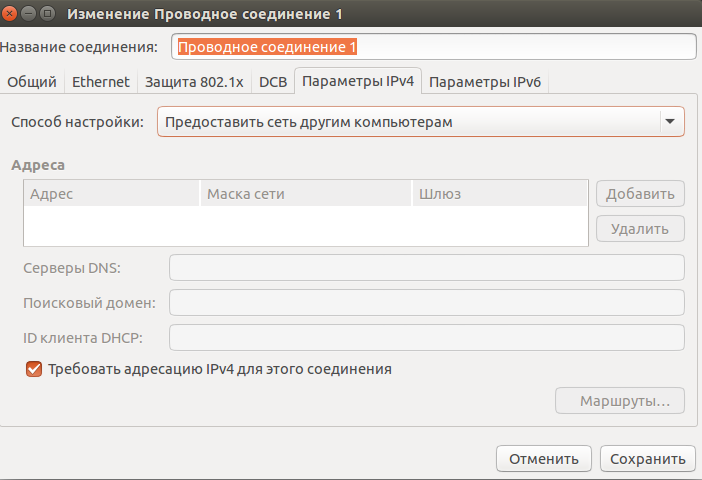
\includegraphics[width=0.6\linewidth]{network_1}}
\caption{ Параметры IPv4 для проводного соединения }
\label{network_1:network_1}
\end{figure}


\begin{figure}[h!]
\center{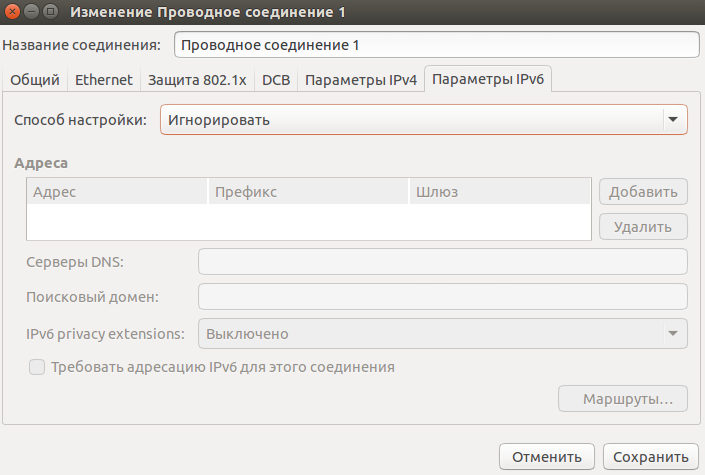
\includegraphics[width=0.6\linewidth]{network_2}}
\caption{ Параметры IPv6 для проводного соединения }
\label{network_2:network_2}
\end{figure}

\begin{figure}[h!]
\center{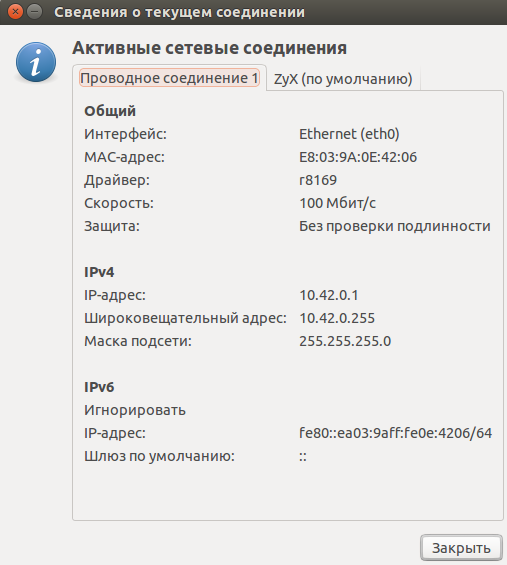
\includegraphics[width=0.6\linewidth]{network_3}}
\caption{ Параметры IPv4 для беспроводного соединения }
\label{network_3:network_3}
\end{figure}

\begin{figure}[h!]
\center{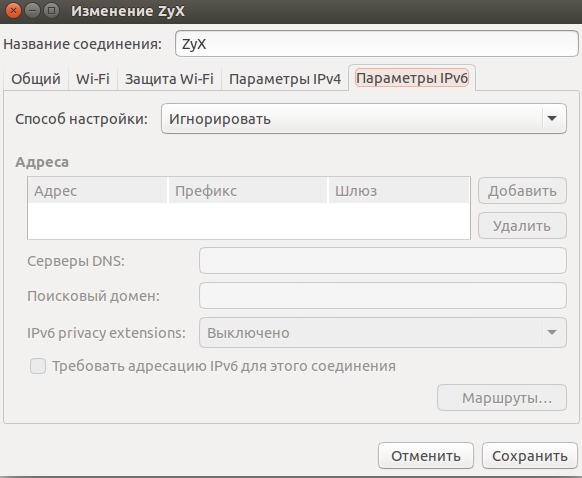
\includegraphics[width=0.6\linewidth]{network_4}}
\caption{ Параметры IPv6 для беспроводного соединения }
\label{network_4:network_4}
\end{figure}

Все остальные настройки оставить по умолчанию.


\begin{figure}[h!]
\center{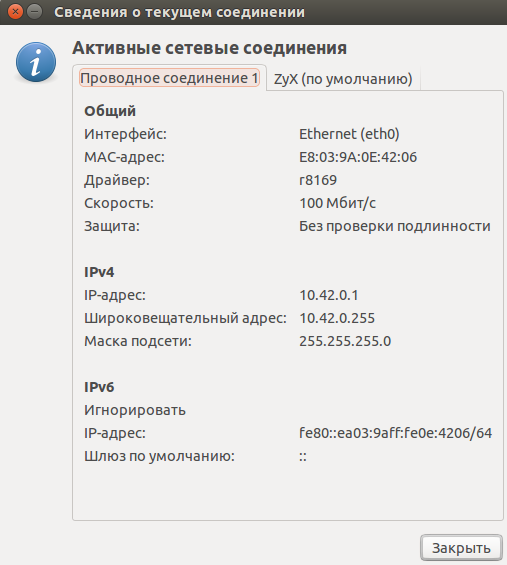
\includegraphics[width=0.6\linewidth]{network_5}}
\caption{ Сведения о проводном соединении }
\label{network_5:network_5}
\end{figure}

\begin{figure}[h!]
\center{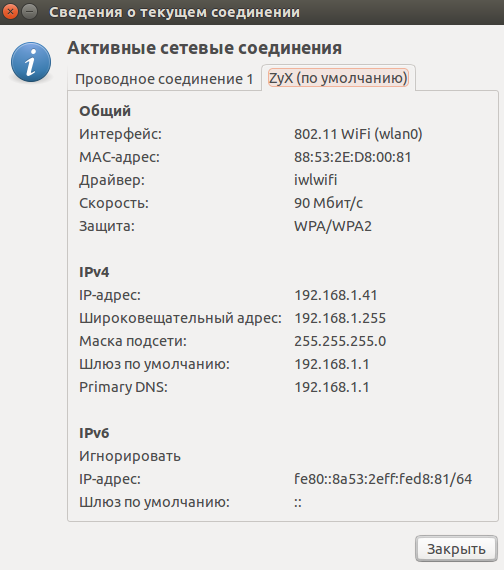
\includegraphics[width=0.6\linewidth]{network_6}}
\caption{ Сведения о беспроводном соединении }
\label{network_6:network_6}
\end{figure}



\clearpage






\subsection{Установка ssh-соединения}


arp -vn:


\begin{figure}[h!]
\center{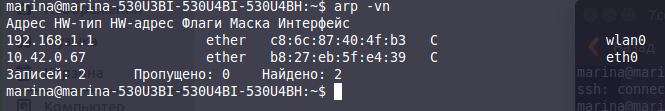
\includegraphics[width=0.6\linewidth]{ssh_1}}
\caption{ Параметры IPv4 для проводного соединения }
\label{ssh_1:ssh_1}
\end{figure}

connect ssh:

\begin{figure}[h!]
\center{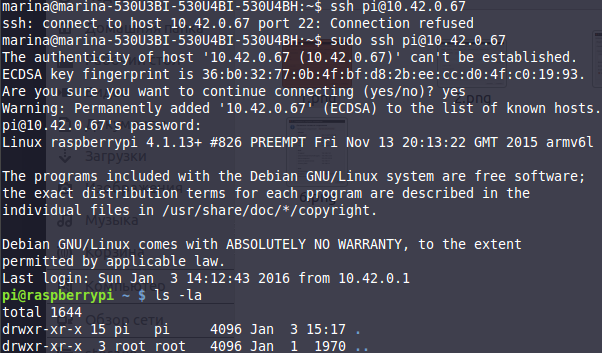
\includegraphics[width=0.6\linewidth]{ssh_2}}
\caption{ Параметры IPv4 для проводного соединения }
\label{ssh_2:ssh_2}
\end{figure}

все,мы в системе

\clearpage

\subsection{Установка драйвера TP-Link}


Узнаем версию системы и проверяем устройства USB

\begin{figure}[h!]
\center{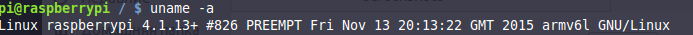
\includegraphics[width=0.8\linewidth]{driver_1}}
\caption{ Узнаем версию системы }
\label{driver_1:driver_1}
\end{figure}


\begin{figure}[h!]
\center{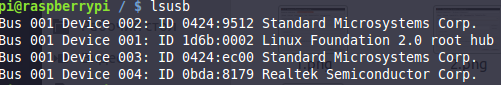
\includegraphics[width=0.6\linewidth]{driver_2}}
\caption{ проверяем устройства USB }
\label{driver_2:driver_2}
\end{figure}


тут ссылка на то,как устанавливать драйвер согласно версии системы
https://www.raspberrypi.org/forums/viewtopic.php?p=462982

Скачиваем драйвер:

\begin{figure}[h!]
\center{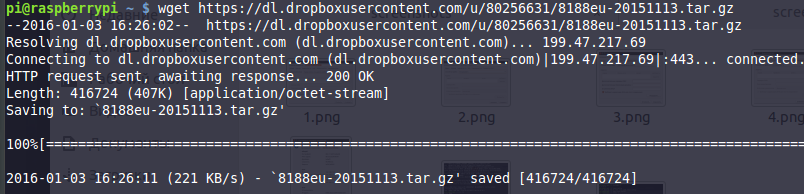
\includegraphics[width=0.8\linewidth]{driver_3}}
\caption{ Скачиваем драйвер }
\label{driver_3:driver_3}
\end{figure}

установим и ребутнемся

\begin{figure}[h!]
\center{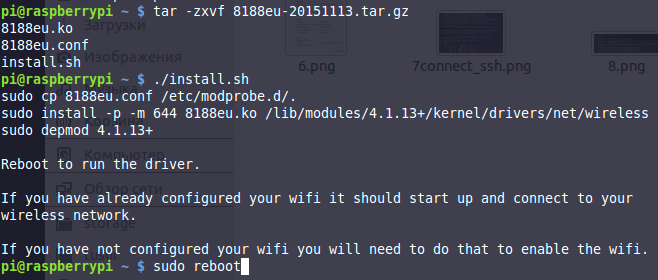
\includegraphics[width=0.7\linewidth]{driver_4}}
\caption{ Устанавливаем драйвер }
\label{driver_4:driver_4}
\end{figure}

Проверим командой ifconfig

\begin{figure}[h!]
\center{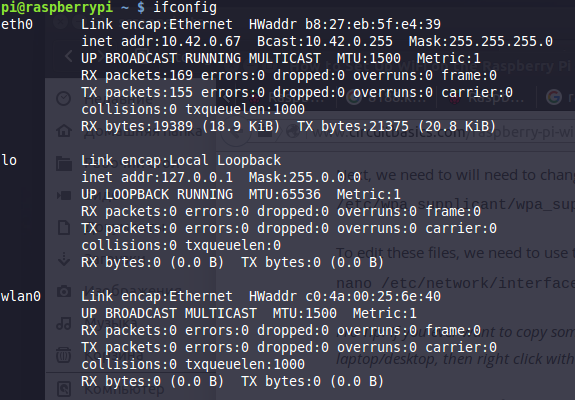
\includegraphics[width=0.6\linewidth]{driver_5}}
\caption{ ifconfig }
\label{driver_5:driver_5}
\end{figure}







\subsection{Настройка режима monitor mode}
Для начала попробуем установить Wi-Fi соединение и подсоединиться к RPi без Ethernet-соединения. 

\begin{figure}[h!]
\center{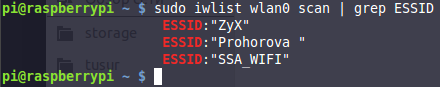
\includegraphics[width=0.6\linewidth]{mm_1}}
\caption{ просканировали сеть }
\label{mm_1:mm_1}
\end{figure}


\begin{figure}[h!]
\center{
\includegraphics[width=0.6\linewidth]{mm_2}}
\caption{ путь к config }
\label{mm_2:mm_2}
\end{figure}


\begin{figure}[h!]
\center{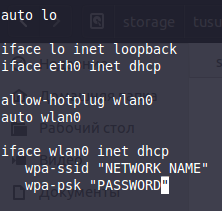
\includegraphics[width=0.3\linewidth]{mm_3}}
\caption{ config }
\label{mm_3:mm_3}
\end{figure}


\begin{figure}[h!]
\center{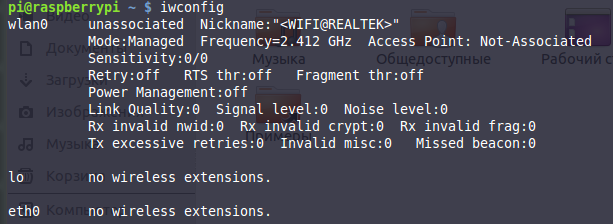
\includegraphics[width=0.7\linewidth]{mm_4}}
\caption{ config }
\label{mm_4:mm_4}
\end{figure}

подняли сетку в режиме Managed

\begin{figure}[h!]
\center{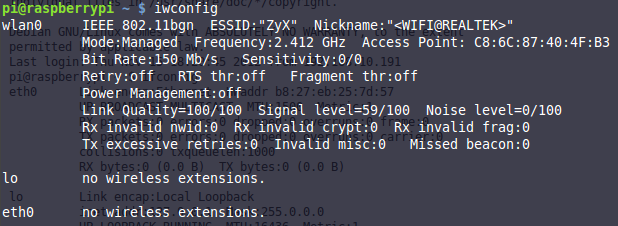
\includegraphics[width=0.7\linewidth]{mm_5}}
\caption{ config }
\label{mm_5:mm_5}
\end{figure}


тут можно рассказать про разные режимы даптеров (их 6) и про мониторящий режим. Устройство может в определенный момент времени находиться только в одном режиме.

Настроим адаптер в режим приема пакетов. Для этого необходимо ввести команду 
sudo iwconfig wlan0 mode monitor
При попытке ввести данную команду видим следующее сообщение:


\begin{figure}[h!]
\center{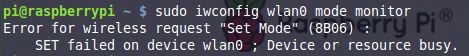
\includegraphics[width=0.6\linewidth]{mm_6}}
\caption{ ресурс занят }
\label{mm_6:mm_6}
\end{figure}

это связано с тем, что в системе работает network interface plugging daemon (ссылка на распберри пи орг)
необходимо его отключить для того, чтобы перевести устройство в другой режим работы

напишем небольшой bash-скрипт, который будет переводить адаптер в режим перехвата пакетов и содержать следующие команды:
sudo service ifplugd stop #останавливаем работу демона
sudo ifconfig wlan0 down #отключаем wi-fi соединение
sudo iwconfig wlan0 mode monitor #включаем прослушивающий режим
sudo ifconfig wlan0 up #включаем wi-fi соединение
sudo service ifplugd start #запускаем демона
iwconfig #проверям настройки

результат работы скрипта приведен на рисунке ... Устройство теперь в режиме перехвата пакетов. Данный скрипт необходимо запускать снова при перезапуске системы, поскольку по умолчанию устройство переходит в режим managed 

\begin{figure}[h!]
\center{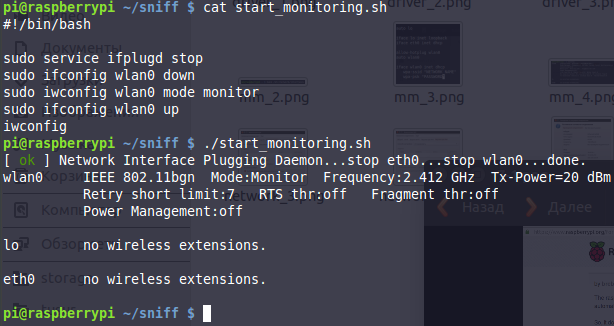
\includegraphics[width=0.6\linewidth]{mm_7}}
\caption{ результат выполнения скрипта }
\label{mm_7:mm_7}
\end{figure}

\clearpage








\subsection{tcpdump}
%\input{technical_things/git}
\subsection{wireshark}
%\input{technical_things/git}



% ----


% руководство пользователя
% руководство программиста
% перспективы применения
% заключение

\clearpage
\renewcommand{\refname}{Список использованных источников}
\bibliography{lit}



% \ESKDappendix{Обязательное}{\normalfont Компакт-диск}
% Компакт-диск содержит: 
% \begin{itemize}
% \item электронную версию пояснительной записки в форматах *.tex и *.pdf;
% \item \textbf{актуальную версию программы};
% \item \textbf{???}.
% \end{itemize}

\end{document}
